\section{Direct Detection }
\label{sec:direct}
\ADW{Some introduction and context is needed here. Much of Lina's intro could be moved here.}

\subsection{Baryon Scattering \Contact{Vera}}
\Contributors{Vera, Kim, Lina N., Ethan N.}

\begin{figure}
\centering
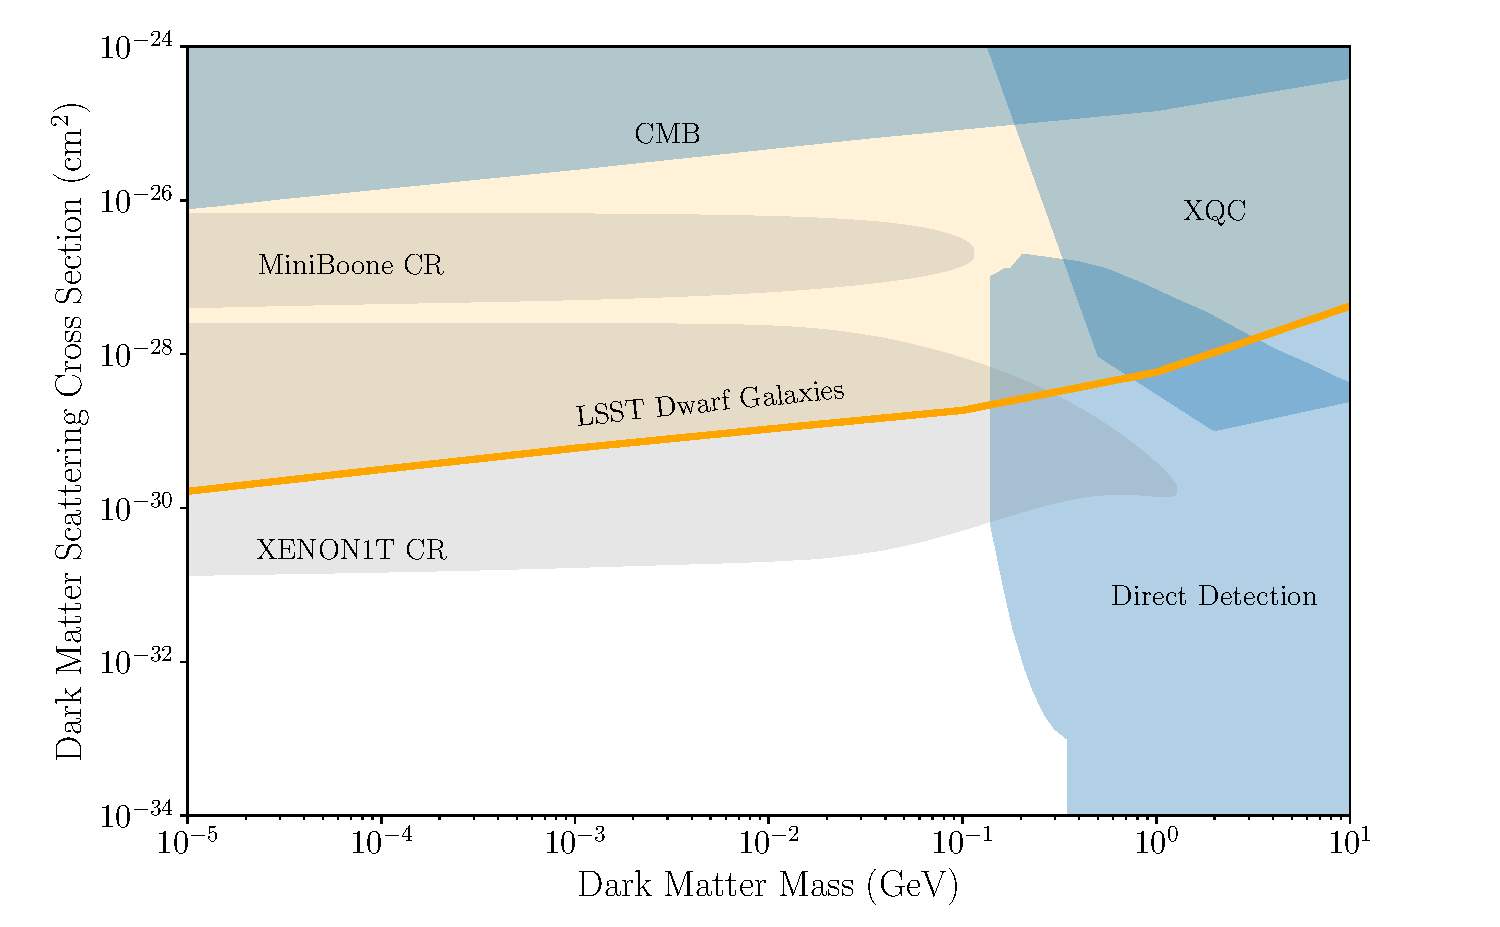
\includegraphics[width=0.75\columnwidth]{bsdm_limits.pdf}
\caption{
Constraints on dark matter-baryon scattering through a velocity-independent, spin-independent contact interaction with protons. 
Existing constraints (shown in blue) include: measurements of the CMB power spectrum \citep[CMB;][]{Gluscevic:2017ywp}, constraints from the X-ray Quantum Calorimeter experiment \citep[XQC;][]{0704.0794}, and direct detection constraints include results from CRESST-III \citep{1711.07692}, the CRESST 2017 surface run \citep{1707.06749}, and XENON1T \citep{1705.06655}, as interpreted by \citet[][]{1802.04764}. %\citep{2018PhRvD..97l3013K}.
Additional constraints that include the effects of cosmic-ray heating of dark matter are shown in gray \citep[][]{1810.10543}.
The projected sensitivity of LSST to dark matter-baryon scattering through observations of Milky Way satellite dwarf galaxies is shown in gold.
}
\label{fig:dd}
\end{figure}

The most sensitive direct searches for dark matter seek to detect the scattering of dark matter particles from the local Galactic halo in underground detectors \citep[\eg][]{1509.08767}. 
They have unprecedented sensitivity to WIMPs with masses above a GeV, but are limited by kinematics when searching for lighter particles. 
New experimental techniques are being explored to directly search for sub-GeV models of dark matter \citep{Battaglieri:2017aum}. 
However, due to atmospheric and terrestrial shielding, most direct dark matter experiments are largely insensitive to dark matter particles with large scattering cross sections. 
Current null results from conventional direct detection experiments motivate broad searches in parameter space that is largely inaccessible to underground experiments. 

%This has motivated a number of experimental tests using astrophysical and cosmological measurements including the X-ray Quantum Calorimeter experiment \citep[XQC;][]{0704.0794} and studies of dark matter-cosmic-ray interactions \citep{Cappiello:2018hsu,1810.10543}.

Cosmological and astrophysical observables are sensitive to scattering of sub-GeV particles with baryons at any point in cosmic history. 
These observations can constrain the interaction cross section to arbitarily high values and are not subject to uncertainties on the local astrophysical properties of dark matter particles \citep[\eg][]{1210.2721,1404.1938}. 
If dark matter particles scatter with baryons, they will transfer momentum between the two cosmological fluids, affecting density fluctuations and suppressing power at small scales. 
This power suppression can be captured by a variety of observables including measurements of the CMB \citep{1311.2937,Gluscevic:2017ywp} and the Lyman-$\alpha$ forest \citep{Xu:2018efh}.
Assuming a velocity-independent, spin-independent contact interaction, cosmological constraints can be directly compared against those from direct detection experiments \citep[\eg][]{Boddy:2018kfv}.
In \figref{dd}, we compare existing constraints on dark matter-baryon scattering from analyses of the CMB and direct-detection searches.\footnote{We caution the reader that this figure does not include a comprehensive list of current constraints, but rather serve to illustrate complementarity of cosmological and direct detection probes.} 
To estimate the future sensitivity of LSST, we map the projected WDM constraints presented in \secref{smallest_galaxies} to a dark matter-baryon scattering constraints by matching the characteristic cutoff scale in the matter power spectrum probed by the lowest-mass subhalos LSST can detect via observations of Milky Way satellite galaxies. 
LSST will deliver measurements of observables that trace matter fluctuations on even smaller scales (\eg, stellar stream gaps), which will potentially extend the sensitivity of these astrophysical and cosmological searches even farther beyond the reach of Planck.


\subsection{Local Dark Matter Velocity Distribution \Contact{Lina}}
\Contributors{Lina N.}

%One way to detect dark matter (DM) is a process called direct detection, where DM particles scatter off heavy nuclei, emitting scintillation/ionization light that provide a direct signal of DM \citep{Goodman:1984dc}. 

The signal strength of dark matter (DM) scattering in direct detection experiments depends on both the local DM density and the DM velocity distribution. In this section we focus on the DM velocity distribution.

The differential rate with respect to the recoil energy $dR/dQ$ depends on the integral of the DM velocity distribution, $f(v)$, as
\begin{equation}
    \frac{dR}{dQ} \propto \int_{v_{\rm{min}}}^{v_{\rm{esc}}} \frac{f(v)}{v} dv, 
\end{equation}
where $v_{\rm{min}} = \sqrt{Q m_N/ (2 \mu^2)}$, with $Q$ the recoil energy, $m_N$ the mass of the nucleus against which DM is scattering, and $\mu = (m_N m_\chi / (m_N + m_\chi))$ the reduced mass of the nucleus $m_N$ and the DM mass $m_\chi$.

A novel method has recently been proposed to use the stars as tracers for the DM velocity \citep{Herzog-Arbeitman:2017fte,Necib:2018b}. These papers suggest that since accreted DM and stars have a comment origin, and are both collisionless, accreted stars are able to trace the velocity distribution of DM. This correlation holds for both the relaxed component of the DM, traced by older metal poor stars, and DM velocity substructure called debris flow traced by less metal poor stars from more recent mergers \citep{Lisanti:2011as,Kuhlen:2012fz,Lisanti:2014dva}. 

This method has already been applied on RAVE-TGAS data \citep{Herzog-Arbeitman:2017zbm}, and the second data release of Gaia in \cite{necib2018}. It has been found that the relaxed component of the DM although isotropic, has a mean speed lower than that of the assumed Maxwell Boltzmann distribution, reducing current limits by direct detection experiments \citep{Aprile:2018dbl}.

Another interesting aspect is the ability to reconstruct of more recent mergers. Using the second data release of Gaia, a new merger called the Gaia Sausage or the Gaia Enceleadus \citep{2018MNRAS.477.1472B,2018Natur.563...85H} has been found. Using the correlation observed in simulations, \cite{necib2018} extracted the new velocity distribution of DM brought in by the same merger, and studied its implications in current direct detection experiments. 

In order to do obtain the full empirical distribution of DM, one needs the 3-d velocities of the stars in the local neighborhood. Gaia provides proper motion and parallaxes for stars down to 20th magnitude. LSST will be able to extend this dataset to fainter stars, giving us a more accurate measurement of proper motions of stars in the solar neighborhood and beyond.

 Using proper motions of stars from LSST, coupled with radial velocity measurements from future telescopes like MSE, we will be able to obtain the most accurate 3-d velocity measurements of the local stars, and subsequently use this information to obtain a full empirical measurement of DM. Such detailed analysis will unveil new structures much smaller than the Gaia Sausage, but with equal importance in DM direct detection if it passes by the Solar neighborhood.
